\documentclass[11pt]{article}
\usepackage{fancyhdr}
\usepackage{tocloft}
\usepackage{graphicx}
\usepackage{calc}
\usepackage{amssymb}
\usepackage{color}
\usepackage[sc]{mathpazo}
\usepackage{url}
\usepackage{ifpdf}
\usepackage{bbding}
\usepackage{caption}
\usepackage{framed}
\usepackage{xcolor}
\usepackage{float}
\usepackage{wrapfig}
\usepackage{sidecap}
\usepackage{multirow}
\linespread{1.0}
\oddsidemargin=0pt
\evensidemargin=0pt
\textwidth=6.5in
\topmargin=0pt
\headheight=0pt
\headsep=0pt
\textheight=9in
\setlength{\parindent}{0.25cm}
\newcommand\secfont{\fontfamily{cmss}\selectfont}%\textwidth 5.5truein
\newcommand\pifheading[1]{\noindent{\secfont\textbf{#1}:}}
\newcommand\yr{2016}
\def\lo{
\mathrel{\raise.3ex\hbox{$<$}\mkern-14mu\lower0.6ex\hbox{$\sim$}}
}
\def\hi{
\mathrel{\raise.3ex\hbox{$>$}\mkern-14mu\lower0.6ex\hbox{$\sim$}}
}

\textwidth = 6.5 in
\textheight = 9 in
\oddsidemargin = -0.00 in
\evensidemargin = +0.05 in
\topmargin = 0 in
\headheight = 0.0 in
\headsep = 0.0 in
\parskip = 0.05in

\newcommand\registered{{\ooalign{\hfil\raise .00ex\hbox{\scriptsize R}\hfil\crcr\mathhexbox20D}}}

%% Define a new 'leo' style for the package that will use a smaller font.
\makeatletter
\def\url@leostyle{%
  \@ifundefined{selectfont}{\def\UrlFont{\sf}}{\def\UrlFont{\small\ttfamily}}}
\makeatother
%% Now actually use the newly defined style.
\urlstyle{leostyle}
\newcommand\checkme[1]{\textcolor{blue}{\textbf{#1}}}
\newcounter{hours}\newcounter{minutes}
\newcommand\printtime{\setcounter{hours}{\time/60}\setcounter{minutes}{\time - \value{hours}*60}\thehours :\theminutes}
\newenvironment{packed_item}{
\begin{itemize}
 \setlength{\itemsep}{1pt}
 \setlength{\parskip}{0pt}
 \setlength{\parsep}{0pt}
}{\end{itemize}}

\newenvironment{packed_enum}{
\begin{enumerate}
 \setlength{\itemsep}{1pt}
 \setlength{\parskip}{0pt}
 \setlength{\parsep}{0pt}
}{\end{enumerate}}

\newenvironment{box_list}{
\begin{itemize}
 \setlength{\itemsep}{3pt}
 \setlength{\parskip}{0pt}
 \setlength{\parsep}{0pt}
}{\end{itemize}}

\newenvironment{packed_list}{
\begin{list}{\labelitemi}{\leftmargin=1em}
 \setlength{\itemsep}{3pt}
 \setlength{\parskip}{0pt}
 \setlength{\parsep}{0pt}
}{\end{list}}

\renewenvironment{quote}{%
  \list{}{%
    \leftmargin10pt   % this is the adjusting screw
    \rightmargin\leftmargin
  }
  \item\relax
}
{\endlist}

% definition of a new float type (refer to the caption package documentation)
\DeclareCaptionType{boxcaption}[Box]
\captionsetup[boxcaption]{position=top,labelfont=bf}

% definition of a shaded-like environment (see framed.sty)
\newenvironment{shadedframe}
  {\def\FrameCommand{\setlength\fboxsep{10pt}\fcolorbox{black}{shadecolor}}%
    \MakeFramed {\advance\hsize-\width \FrameRestore}}%
{\endMakeFramed}

\newenvironment{shadedbox}{%
  \def\FrameCommand{\colorbox{shadecolor}}%
  \MakeFramed {\FrameRestore}}%
 {\endMakeFramed}

% main environment
% syntax: \begin{myenv}{placement-specifiers}{color}{width}...\end{myenv}
\newenvironment{boxenv}[3]
  {\colorlet{shadecolor}{#2}%
    \begin{boxcaption}[#1]%
    \noindent\begin{minipage}{#3}
      \begin{shadedframe}
      }
  {\end{shadedframe}\end{minipage}\end{boxcaption}}

 % TOC
\usepackage{enumerate}
\begin{document}


\begin{figure}
  
\includegraphics[width=\linewidth/3]{title}
  \label{fig:title}
\end{figure}


\title{Lab Report 9: Digital Electronics The Basics}


\author{Yuezhe Yao}

%\institute{Syracuse University}



\maketitle

\begin{abstract}
In this lab, we utilized LabVIEW and the digital functions of our DAQ card to learn some of the basics of digital electronics and operate several important digital components.      
\end{abstract}

\medskip

\begingroup
\let\clearpage\relax
\tableofcontents
\endgroup

\medskip
\medskip

\section{Learning Objectives}


To become familiar with basic digital concepts and terminology 

To become familiar with the digital input/output (I/O) functions of LabVIEW and the NI USB-6003

To learn about important digital circuit elements like gates, flip-flops, timers, counters, and registers

To gain appreciation of how digital circuits shape our modern world

\section{Activity I - Basic Introduction to Digital Concepts \& Termin
ology}


For 3-input NAND, except the condition when all the 3 inputs are 1, the output would be 0 then. Otherwise the output would be 1.

A \quad B  \quad  C  \quad X

1  \quad\,  1 \quad 1  \quad\,   0

otherwise \quad \ \, 1

\vbox{}

For 2-input XOR

A \quad B   \quad \ X

0  \quad\,  0 \quad\,   0

0  \quad\,  1 \quad\,   1

1  \quad\,  0 \quad\,   1

1  \quad\,  1 \quad\,   0

\vbox{}

Yes we were able to reproduce these tables.


\section{Activity II - Digital I/O with LabVIEW and the PCI-6023/24E}


\begin{figure}[H]
 \begin{center}
  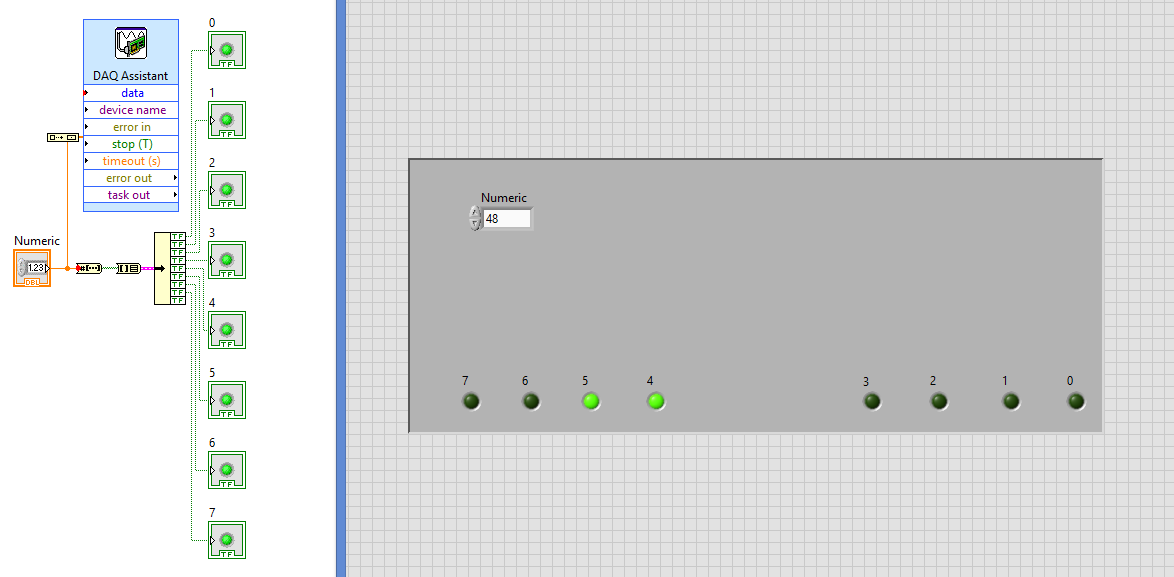
\includegraphics[width=\linewidth/1]{act2_2}
  \caption{The front panel and block diagram of the output of all integers from 1 to 255.}
  \label{fig:act2_2}
 \end{center}
\end{figure}

\begin{figure}[H]
 \begin{center}
  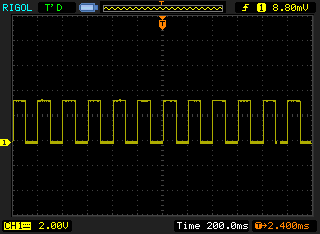
\includegraphics[width=\linewidth/2]{act2_2b}
  \caption{The output of a square TTL wave.}
  \label{fig:act2_2b}
 \end{center}
\end{figure}

\begin{figure}[H]
 \begin{center}
  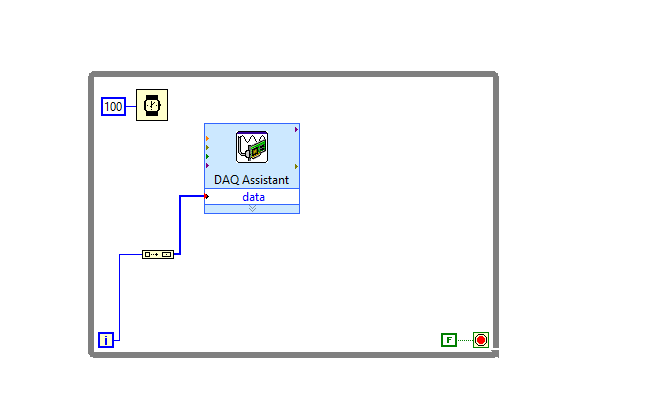
\includegraphics[width=\linewidth/2]{act2_3b}
  \caption{The block diagram of the output of a square TTL wave.}
  \label{fig:act2_3b}
 \end{center}
\end{figure}

\begin{figure}[H]
 \begin{center}
  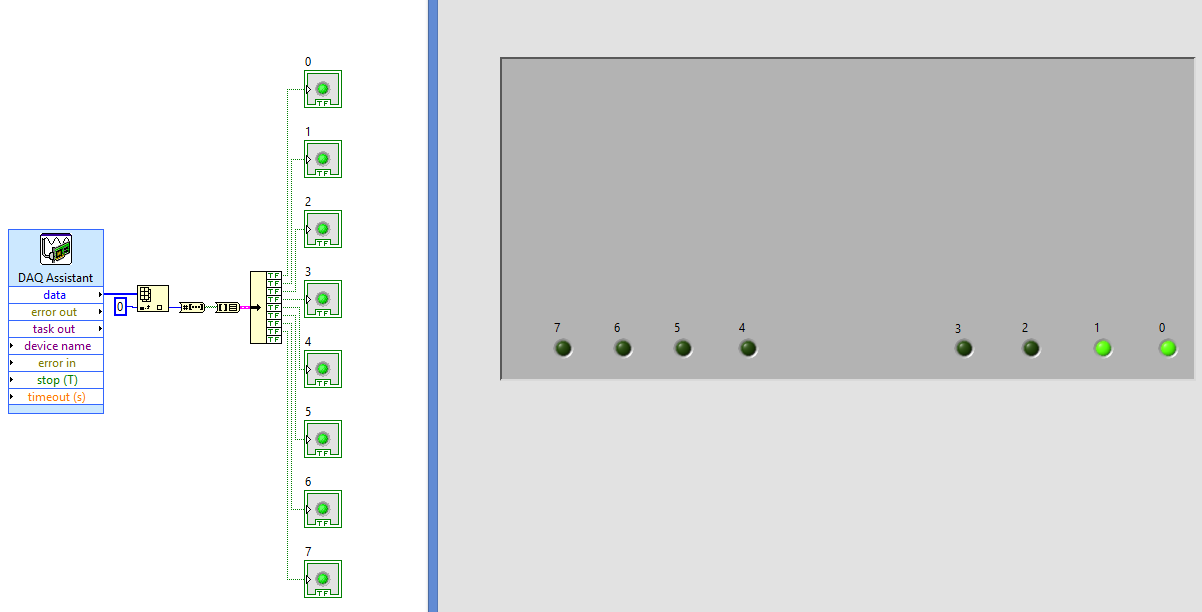
\includegraphics[width=\linewidth/2]{act2_4}
  \caption{The front panel and block diagram of the display of the logic levels on LED indicators.}
  \label{fig:act2_4}
 \end{center}
\end{figure}


\section{Activity III - The 2-Bit Full Adder and Subtractor}


\begin{figure}[H]
 \begin{center}
  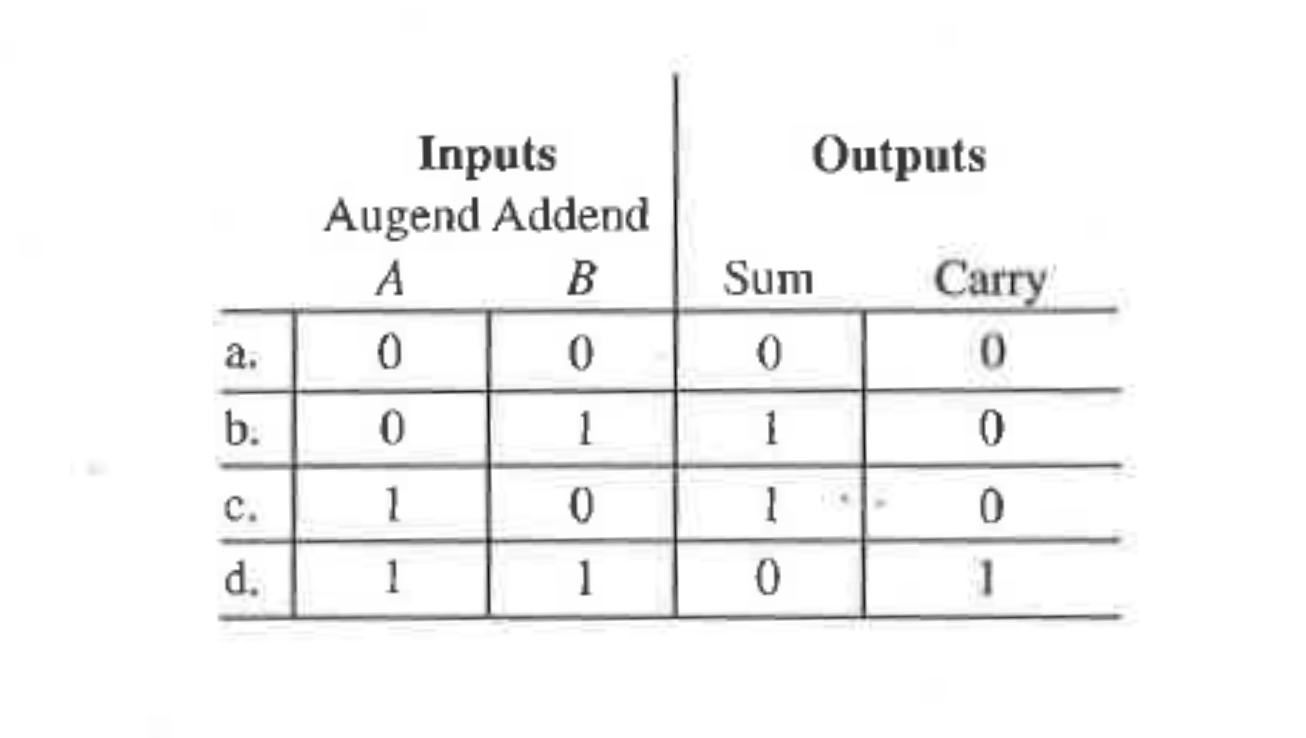
\includegraphics[width=\linewidth/2]{act3}
  \caption{The truth table the full adder.}
  \label{fig:act3}
 \end{center}
\end{figure}

Yes our circuit operated in the manner that we expected.


\section{Activity IV - Flip-Flops}

\begin{figure}[H]
 \begin{center}
  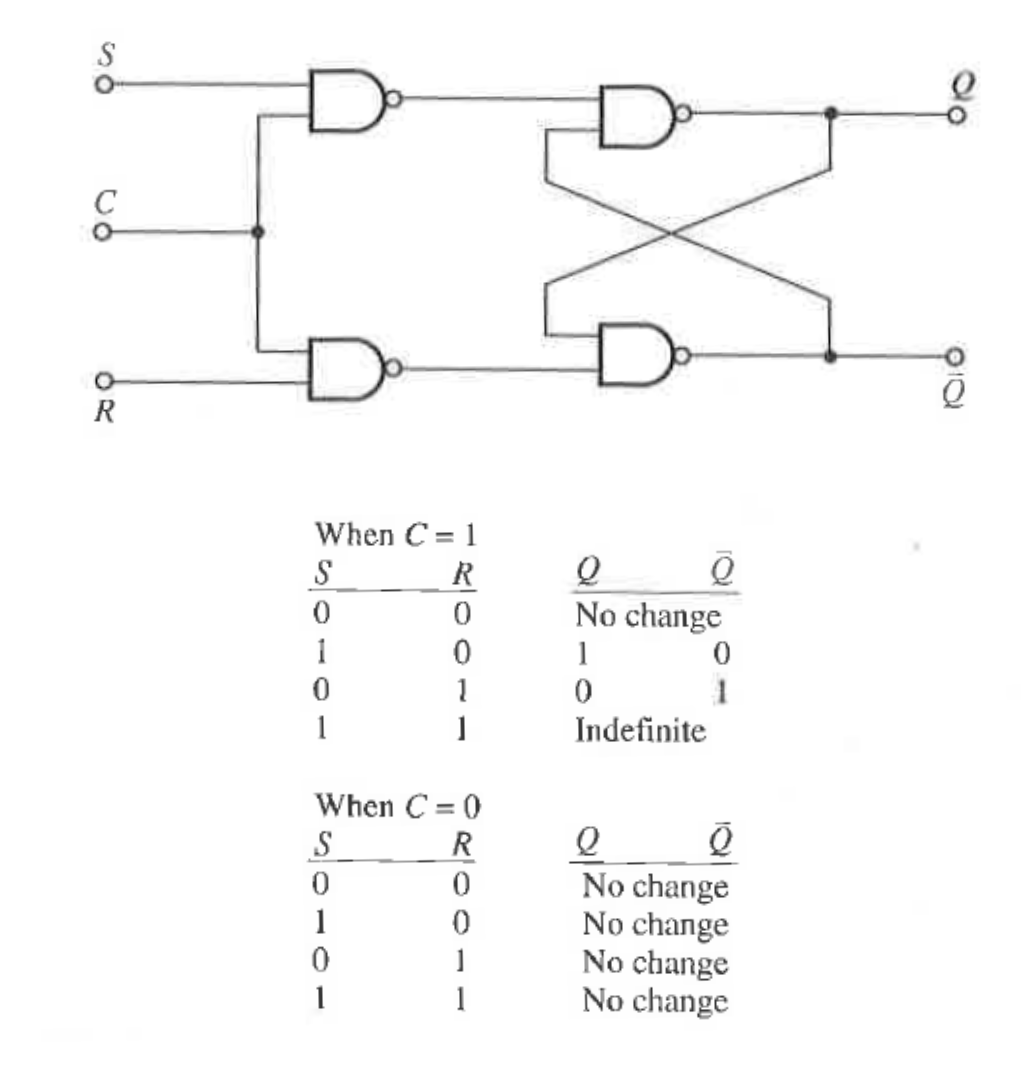
\includegraphics[width=\linewidth/2]{act4rsff}
  \caption{RSFF.}
  \label{fig:act4rsff}
 \end{center}
\end{figure}

For the clocked RSFF and DFF:

Everything went well and we successfully get the right truth table as shown above, except that the 74HC03N (four 2-input NAND) doesn't work well. We found that its voltage is about 3V, so either the green light (for low output voltage) nor the red light (for high output voltage) were on. So we use the 74HC10N (3-input NAND) instead (just set the C-input as the high voltage).

\vbox{}

For the clocked TSFF, when $C = 0, Q =\overline{\bar{Q}\cdot 1} = Q$, and the same happens to $\bar{Q}$, so they will not change as S or R change. When C = 1 and $R = S = 0, Q = \overline{\bar{Q}\cdot1} = Q$. But if R and S both change to 1 while C = 1, Q and $\bar{Q}$ all should equal to 1, which does not fit the purpose of the circuit.

\vbox{}

For the DFF, the mechanism of it is same as the clocked TSFF's. When CLK=1, Q=S=DATA.

\vbox{}

For TFF:


\begin{figure}[H]
 \begin{center}
  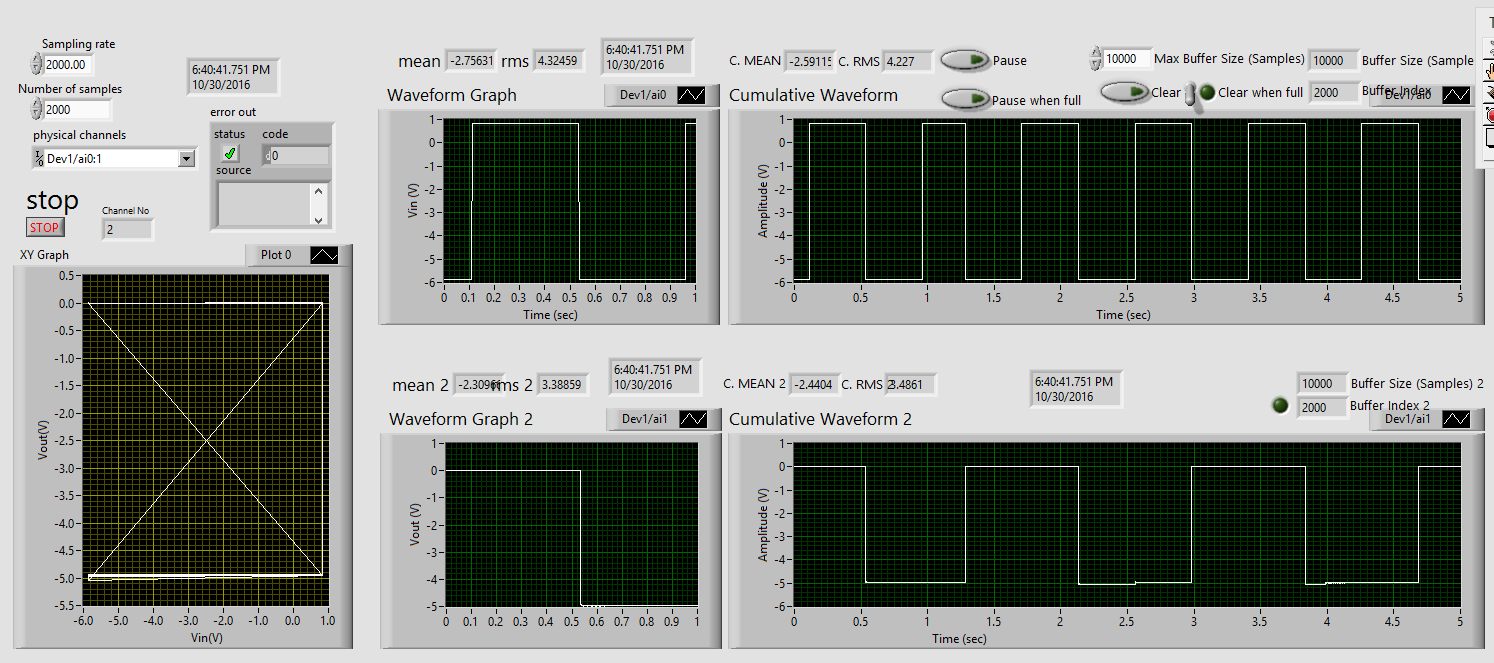
\includegraphics[width=\linewidth/1]{act4_3}
  \caption{The front panel of the TTF.}
  \label{fig:act4_3}
 \end{center}
\end{figure}

We constructed one and tested it by 1Hz TTL signal. In the first RSFF of the TFF, the first pulse of $CLK_{1}$ changed $Q_{1}$ when $Q_{2}$ keeps its value because $CLK_{2} = CLK_{1} = 0$. After $CLK_{1}$ changes to 0, $CLK_{2} = 1$ so $Q_{2} = Q_{1}$. Therefore $Q_{2}$ flips its value once every CLK period and twice every 2 CLK periods, which means $f_{Q} = \frac{f_{CLK}}{2}$.


\begin{figure}[H]
 \begin{center}
  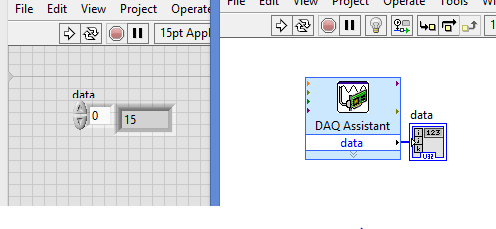
\includegraphics[width=\linewidth/2]{act4_4}
  \caption{The front panel and the block diagram of the count-to-16 counter.}
  \label{fig:act4_4}
 \end{center}
\end{figure}

We used 4 JKFFs to build our count-to-16 circuit. The J and K inputs on each of the JKFFs are set to one, so the JKFFs each act as TFFs. As a result of this, the second JKFF undergoes one toggle in output value for every two toggles of the output of the first JKFF. In this manner, the first LED should flash at the frequency $f_{1} = \frac{f_{CLK}}{2}$ , the second flashes at $f_{2} = \frac{f_{1}}{2}$ and so on. Additionally, for each input clock cycle a binary number is produced by the two cells (JKFFs). For the count-to-16 counter the  numbers  cycle sequentially between 0 and 15.  

\vbox{}

Then we used LabVIEW to record the operation of the shift-register in real-time the LED logic indicators on the 503 board. And we showed the instructor our results. For the shift-register, as shown in the picture below, all JKFFs are initialized with output equal to zero (A=B=C=D=0).  
Then a pulse (a one) is sent into the Data terminal. On the next positive clock edge, this toggles the output of the first JKFF to one (A=1). The output A is fed into terminal J of the second JKFF. Then on the next 
positive clock edge, the output of the second JKFF toggles to one (B=1). And so on, until the data is transferred to the end of the register.

\begin{figure}[H]
 \begin{center}
  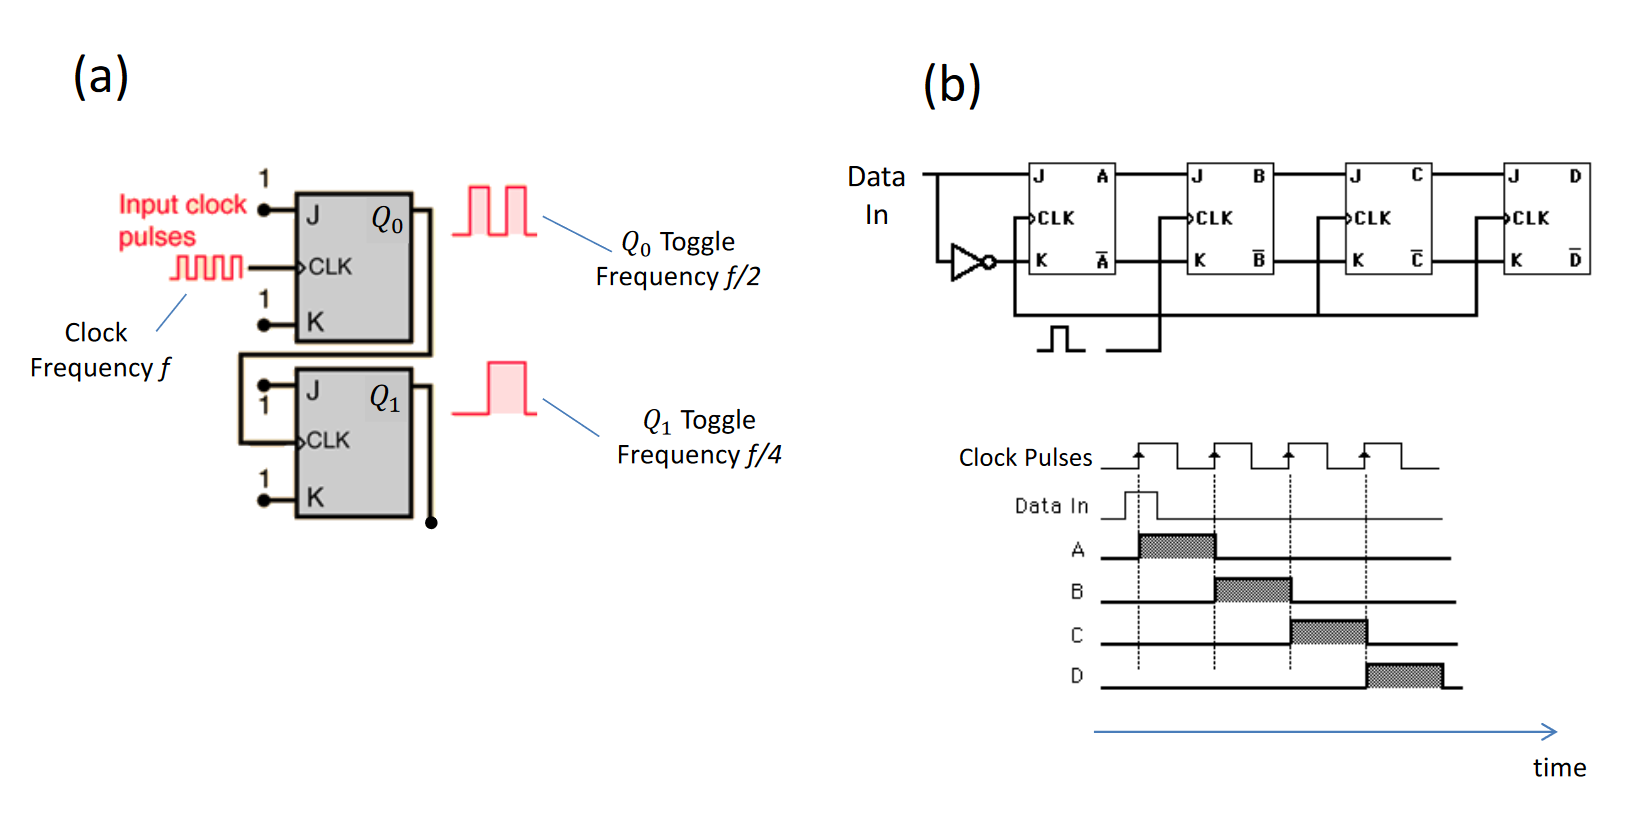
\includegraphics[width=\linewidth/2]{act4_6}
  \caption{(a)Schematic of a 2-bit binary counter.(b)Schematic of a 4-bit serial shift register.}
  \label{fig:act4_6}
 \end{center}
\end{figure}





\end{document}
